
\noindent\textbf{18. (CLRS 24.3-2)} Mostre que o algoritmo de Dijkstra pode produzir resultados errados se o dígrafo tiver arcos de custo estritamente negativo.\\[6pt]
\textbf{Resposta:} Um exemplo para dígrafos pode ser visto na figura \ref{fig:8.18-1}.

\begin{center}
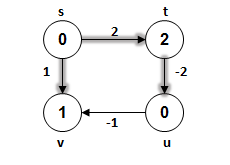
\includegraphics[width=0.35\textwidth]{q8-18.png}
\captionof{figure}{Dígrafo com arcos estritamente negativos.}
\label{fig:8.18-1}
\end{center}

A execução de todas as iterações do \proc{Dijkstra} produz o caminho mínimo destacado pelas arestas sombreadas. O valor de $d[v]$ está errado, pois existe um caminho mínimo de $s \leadsto v$ de custo menor que 1, por exemplo, o caminho $p' = s \leadsto t \leadsto u \leadsto v$, onde $w(p') = -1 < 1$.